% Created by tikzDevice version 0.11 on 2018-04-12 15:36:09
% !TEX encoding = UTF-8 Unicode
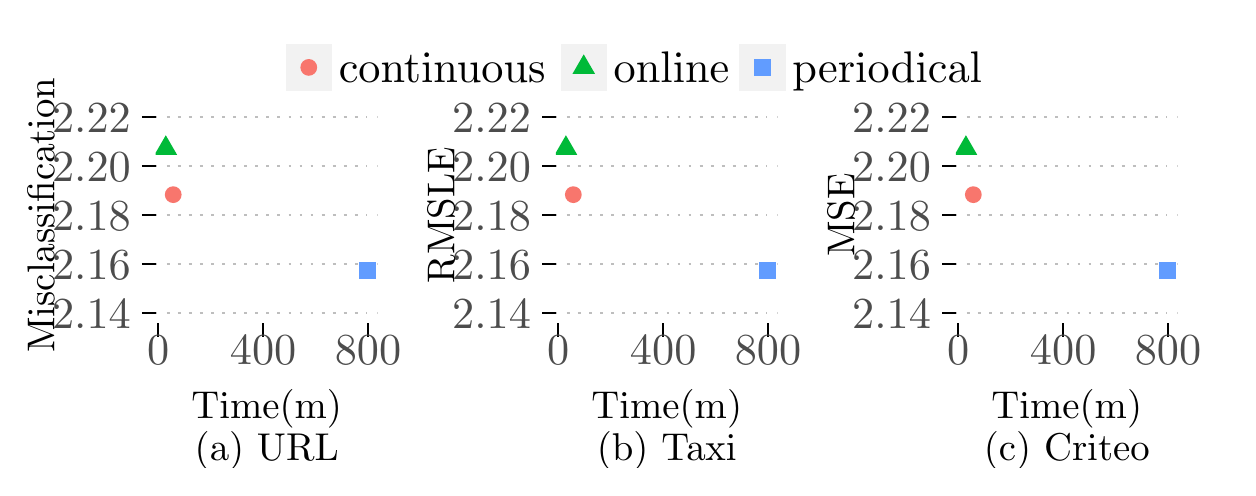
\begin{tikzpicture}[x=1pt,y=1pt]
\definecolor{fillColor}{RGB}{255,255,255}
\path[use as bounding box,fill=fillColor,fill opacity=0.00] (0,0) rectangle (433.62,158.99);
\begin{scope}
\path[clip] (  0.00,  0.00) rectangle (433.62,158.99);
\definecolor{fillColor}{RGB}{255,255,255}

\path[fill=fillColor] ( 82.87,130.27) rectangle (350.75,158.99);
\end{scope}
\begin{scope}
\path[clip] (  0.00,  0.00) rectangle (433.62,158.99);
\definecolor{drawColor}{RGB}{0,0,0}

\node[text=drawColor,anchor=base west,inner sep=0pt, outer sep=0pt, scale=  0.00] at ( 88.56,144.63) {Deployment};
\end{scope}
\begin{scope}
\path[clip] (  0.00,  0.00) rectangle (433.62,158.99);
\definecolor{drawColor}{RGB}{255,255,255}
\definecolor{fillColor}{gray}{0.95}

\path[draw=drawColor,line width= 0.6pt,line join=round,line cap=round,fill=fillColor] ( 92.90,135.96) rectangle (110.24,153.30);
\end{scope}
\begin{scope}
\path[clip] (  0.00,  0.00) rectangle (433.62,158.99);
\definecolor{fillColor}{RGB}{248,118,109}

\path[fill=fillColor] (101.57,144.63) circle (  3.03);
\end{scope}
\begin{scope}
\path[clip] (  0.00,  0.00) rectangle (433.62,158.99);
\definecolor{drawColor}{RGB}{255,255,255}
\definecolor{fillColor}{gray}{0.95}

\path[draw=drawColor,line width= 0.6pt,line join=round,line cap=round,fill=fillColor] (192.26,135.96) rectangle (209.60,153.30);
\end{scope}
\begin{scope}
\path[clip] (  0.00,  0.00) rectangle (433.62,158.99);
\definecolor{fillColor}{RGB}{0,186,56}

\path[fill=fillColor] (200.93,149.35) --
	(205.02,142.27) --
	(196.85,142.27) --
	cycle;
\end{scope}
\begin{scope}
\path[clip] (  0.00,  0.00) rectangle (433.62,158.99);
\definecolor{drawColor}{RGB}{255,255,255}
\definecolor{fillColor}{gray}{0.95}

\path[draw=drawColor,line width= 0.6pt,line join=round,line cap=round,fill=fillColor] (256.80,135.96) rectangle (274.15,153.30);
\end{scope}
\begin{scope}
\path[clip] (  0.00,  0.00) rectangle (433.62,158.99);
\definecolor{fillColor}{RGB}{97,156,255}

\path[fill=fillColor] (262.44,141.60) --
	(268.51,141.60) --
	(268.51,147.66) --
	(262.44,147.66) --
	cycle;
\end{scope}
\begin{scope}
\path[clip] (  0.00,  0.00) rectangle (433.62,158.99);
\definecolor{drawColor}{RGB}{0,0,0}

\node[text=drawColor,anchor=base west,inner sep=0pt, outer sep=0pt, scale=  1.60] at (112.41,139.12) {continuous};
\end{scope}
\begin{scope}
\path[clip] (  0.00,  0.00) rectangle (433.62,158.99);
\definecolor{drawColor}{RGB}{0,0,0}

\node[text=drawColor,anchor=base west,inner sep=0pt, outer sep=0pt, scale=  1.60] at (211.77,139.12) {online};
\end{scope}
\begin{scope}
\path[clip] (  0.00,  0.00) rectangle (433.62,158.99);
\definecolor{drawColor}{RGB}{0,0,0}

\node[text=drawColor,anchor=base west,inner sep=0pt, outer sep=0pt, scale=  1.60] at (276.32,139.12) {periodical};
\end{scope}
\begin{scope}
\path[clip] (  0.00,  0.00) rectangle (144.54,130.27);
\definecolor{drawColor}{RGB}{255,255,255}
\definecolor{fillColor}{RGB}{255,255,255}

\path[draw=drawColor,line width= 0.6pt,line join=round,line cap=round,fill=fillColor] (  0.00,  0.00) rectangle (144.54,130.27);
\end{scope}
\begin{scope}
\path[clip] ( 46.26, 52.27) rectangle (126.47,130.27);
\definecolor{fillColor}{RGB}{255,255,255}

\path[fill=fillColor] ( 46.26, 52.27) rectangle (126.47,130.27);
\definecolor{drawColor}{RGB}{255,255,255}

\path[draw=drawColor,line width= 0.3pt,line join=round] ( 46.26, 64.68) --
	(126.47, 64.68);

\path[draw=drawColor,line width= 0.3pt,line join=round] ( 46.26, 82.41) --
	(126.47, 82.41);

\path[draw=drawColor,line width= 0.3pt,line join=round] ( 46.26,100.13) --
	(126.47,100.13);

\path[draw=drawColor,line width= 0.3pt,line join=round] ( 46.26,117.86) --
	(126.47,117.86);

\path[draw=drawColor,line width= 0.3pt,line join=round] ( 66.11, 52.27) --
	( 66.11,130.27);

\path[draw=drawColor,line width= 0.3pt,line join=round] (104.03, 52.27) --
	(104.03,130.27);
\definecolor{drawColor}{RGB}{190,190,190}

\path[draw=drawColor,line width= 0.6pt,dash pattern=on 1pt off 3pt ,line join=round] ( 46.26, 55.82) --
	(126.47, 55.82);

\path[draw=drawColor,line width= 0.6pt,dash pattern=on 1pt off 3pt ,line join=round] ( 46.26, 73.55) --
	(126.47, 73.55);

\path[draw=drawColor,line width= 0.6pt,dash pattern=on 1pt off 3pt ,line join=round] ( 46.26, 91.27) --
	(126.47, 91.27);

\path[draw=drawColor,line width= 0.6pt,dash pattern=on 1pt off 3pt ,line join=round] ( 46.26,109.00) --
	(126.47,109.00);

\path[draw=drawColor,line width= 0.6pt,dash pattern=on 1pt off 3pt ,line join=round] ( 46.26,126.72) --
	(126.47,126.72);
\definecolor{drawColor}{RGB}{255,255,255}

\path[draw=drawColor,line width= 0.6pt,line join=round] ( 47.15, 52.27) --
	( 47.15,130.27);

\path[draw=drawColor,line width= 0.6pt,line join=round] ( 85.07, 52.27) --
	( 85.07,130.27);

\path[draw=drawColor,line width= 0.6pt,line join=round] (122.99, 52.27) --
	(122.99,130.27);
\definecolor{fillColor}{RGB}{0,186,56}

\path[fill=fillColor] ( 49.91,120.12) --
	( 53.99,113.05) --
	( 45.82,113.05) --
	cycle;
\definecolor{fillColor}{RGB}{248,118,109}

\path[fill=fillColor] ( 52.59, 98.65) circle (  3.03);
\definecolor{fillColor}{RGB}{97,156,255}

\path[fill=fillColor] (119.79, 68.32) --
	(125.86, 68.32) --
	(125.86, 74.39) --
	(119.79, 74.39) --
	cycle;
\end{scope}
\begin{scope}
\path[clip] (  0.00,  0.00) rectangle (433.62,158.99);
\definecolor{drawColor}{gray}{0.30}

\node[text=drawColor,anchor=base east,inner sep=0pt, outer sep=0pt, scale=  1.60] at ( 37.26, 50.31) {2.14};

\node[text=drawColor,anchor=base east,inner sep=0pt, outer sep=0pt, scale=  1.60] at ( 37.26, 68.04) {2.16};

\node[text=drawColor,anchor=base east,inner sep=0pt, outer sep=0pt, scale=  1.60] at ( 37.26, 85.76) {2.18};

\node[text=drawColor,anchor=base east,inner sep=0pt, outer sep=0pt, scale=  1.60] at ( 37.26,103.49) {2.20};

\node[text=drawColor,anchor=base east,inner sep=0pt, outer sep=0pt, scale=  1.60] at ( 37.26,121.21) {2.22};
\end{scope}
\begin{scope}
\path[clip] (  0.00,  0.00) rectangle (433.62,158.99);
\definecolor{drawColor}{RGB}{0,0,0}

\path[draw=drawColor,line width= 0.6pt,line join=round] ( 41.26, 55.82) --
	( 46.26, 55.82);

\path[draw=drawColor,line width= 0.6pt,line join=round] ( 41.26, 73.55) --
	( 46.26, 73.55);

\path[draw=drawColor,line width= 0.6pt,line join=round] ( 41.26, 91.27) --
	( 46.26, 91.27);

\path[draw=drawColor,line width= 0.6pt,line join=round] ( 41.26,109.00) --
	( 46.26,109.00);

\path[draw=drawColor,line width= 0.6pt,line join=round] ( 41.26,126.72) --
	( 46.26,126.72);
\end{scope}
\begin{scope}
\path[clip] (  0.00,  0.00) rectangle (433.62,158.99);
\definecolor{drawColor}{RGB}{0,0,0}

\path[draw=drawColor,line width= 0.6pt,line join=round] ( 47.15, 47.27) --
	( 47.15, 52.27);

\path[draw=drawColor,line width= 0.6pt,line join=round] ( 85.07, 47.27) --
	( 85.07, 52.27);

\path[draw=drawColor,line width= 0.6pt,line join=round] (122.99, 47.27) --
	(122.99, 52.27);
\end{scope}
\begin{scope}
\path[clip] (  0.00,  0.00) rectangle (433.62,158.99);
\definecolor{drawColor}{gray}{0.30}

\node[text=drawColor,anchor=base,inner sep=0pt, outer sep=0pt, scale=  1.60] at ( 47.15, 37.26) {0};

\node[text=drawColor,anchor=base,inner sep=0pt, outer sep=0pt, scale=  1.60] at ( 85.07, 37.26) {400};

\node[text=drawColor,anchor=base,inner sep=0pt, outer sep=0pt, scale=  1.60] at (122.99, 37.26) {800};
\end{scope}
\begin{scope}
\path[clip] (  0.00,  0.00) rectangle (433.62,158.99);
\definecolor{drawColor}{RGB}{0,0,0}

\node[text=drawColor,anchor=base,inner sep=0pt, outer sep=0pt, scale=  1.40] at ( 86.37, 17.61) {Time(m)};

\node[text=drawColor,anchor=base,inner sep=0pt, outer sep=0pt, scale=  1.40] at ( 86.37,  2.49) {(a) URL};
\end{scope}
\begin{scope}
\path[clip] (  0.00,  0.00) rectangle (433.62,158.99);
\definecolor{drawColor}{RGB}{0,0,0}

\node[text=drawColor,rotate= 90.00,anchor=base,inner sep=0pt, outer sep=0pt, scale=  1.40] at (  9.64, 91.27) {Misclassification};
\end{scope}
\begin{scope}
\path[clip] (144.54,  0.00) rectangle (289.08,130.27);
\definecolor{drawColor}{RGB}{255,255,255}
\definecolor{fillColor}{RGB}{255,255,255}

\path[draw=drawColor,line width= 0.6pt,line join=round,line cap=round,fill=fillColor] (144.54,  0.00) rectangle (289.08,130.27);
\end{scope}
\begin{scope}
\path[clip] (190.85, 52.27) rectangle (271.01,130.27);
\definecolor{fillColor}{RGB}{255,255,255}

\path[fill=fillColor] (190.85, 52.27) rectangle (271.01,130.27);
\definecolor{drawColor}{RGB}{255,255,255}

\path[draw=drawColor,line width= 0.3pt,line join=round] (190.85, 64.68) --
	(271.01, 64.68);

\path[draw=drawColor,line width= 0.3pt,line join=round] (190.85, 82.41) --
	(271.01, 82.41);

\path[draw=drawColor,line width= 0.3pt,line join=round] (190.85,100.13) --
	(271.01,100.13);

\path[draw=drawColor,line width= 0.3pt,line join=round] (190.85,117.86) --
	(271.01,117.86);

\path[draw=drawColor,line width= 0.3pt,line join=round] (210.69, 52.27) --
	(210.69,130.27);

\path[draw=drawColor,line width= 0.3pt,line join=round] (248.59, 52.27) --
	(248.59,130.27);
\definecolor{drawColor}{RGB}{190,190,190}

\path[draw=drawColor,line width= 0.6pt,dash pattern=on 1pt off 3pt ,line join=round] (190.85, 55.82) --
	(271.01, 55.82);

\path[draw=drawColor,line width= 0.6pt,dash pattern=on 1pt off 3pt ,line join=round] (190.85, 73.55) --
	(271.01, 73.55);

\path[draw=drawColor,line width= 0.6pt,dash pattern=on 1pt off 3pt ,line join=round] (190.85, 91.27) --
	(271.01, 91.27);

\path[draw=drawColor,line width= 0.6pt,dash pattern=on 1pt off 3pt ,line join=round] (190.85,109.00) --
	(271.01,109.00);

\path[draw=drawColor,line width= 0.6pt,dash pattern=on 1pt off 3pt ,line join=round] (190.85,126.72) --
	(271.01,126.72);
\definecolor{drawColor}{RGB}{255,255,255}

\path[draw=drawColor,line width= 0.6pt,line join=round] (191.74, 52.27) --
	(191.74,130.27);

\path[draw=drawColor,line width= 0.6pt,line join=round] (229.64, 52.27) --
	(229.64,130.27);

\path[draw=drawColor,line width= 0.6pt,line join=round] (267.53, 52.27) --
	(267.53,130.27);
\definecolor{fillColor}{RGB}{0,186,56}

\path[fill=fillColor] (194.49,120.12) --
	(198.58,113.05) --
	(190.41,113.05) --
	cycle;
\definecolor{fillColor}{RGB}{248,118,109}

\path[fill=fillColor] (197.17, 98.65) circle (  3.03);
\definecolor{fillColor}{RGB}{97,156,255}

\path[fill=fillColor] (264.34, 68.32) --
	(270.40, 68.32) --
	(270.40, 74.39) --
	(264.34, 74.39) --
	cycle;
\end{scope}
\begin{scope}
\path[clip] (  0.00,  0.00) rectangle (433.62,158.99);
\definecolor{drawColor}{gray}{0.30}

\node[text=drawColor,anchor=base east,inner sep=0pt, outer sep=0pt, scale=  1.60] at (181.85, 50.31) {2.14};

\node[text=drawColor,anchor=base east,inner sep=0pt, outer sep=0pt, scale=  1.60] at (181.85, 68.04) {2.16};

\node[text=drawColor,anchor=base east,inner sep=0pt, outer sep=0pt, scale=  1.60] at (181.85, 85.76) {2.18};

\node[text=drawColor,anchor=base east,inner sep=0pt, outer sep=0pt, scale=  1.60] at (181.85,103.49) {2.20};

\node[text=drawColor,anchor=base east,inner sep=0pt, outer sep=0pt, scale=  1.60] at (181.85,121.21) {2.22};
\end{scope}
\begin{scope}
\path[clip] (  0.00,  0.00) rectangle (433.62,158.99);
\definecolor{drawColor}{RGB}{0,0,0}

\path[draw=drawColor,line width= 0.6pt,line join=round] (185.85, 55.82) --
	(190.85, 55.82);

\path[draw=drawColor,line width= 0.6pt,line join=round] (185.85, 73.55) --
	(190.85, 73.55);

\path[draw=drawColor,line width= 0.6pt,line join=round] (185.85, 91.27) --
	(190.85, 91.27);

\path[draw=drawColor,line width= 0.6pt,line join=round] (185.85,109.00) --
	(190.85,109.00);

\path[draw=drawColor,line width= 0.6pt,line join=round] (185.85,126.72) --
	(190.85,126.72);
\end{scope}
\begin{scope}
\path[clip] (  0.00,  0.00) rectangle (433.62,158.99);
\definecolor{drawColor}{RGB}{0,0,0}

\path[draw=drawColor,line width= 0.6pt,line join=round] (191.74, 47.27) --
	(191.74, 52.27);

\path[draw=drawColor,line width= 0.6pt,line join=round] (229.64, 47.27) --
	(229.64, 52.27);

\path[draw=drawColor,line width= 0.6pt,line join=round] (267.53, 47.27) --
	(267.53, 52.27);
\end{scope}
\begin{scope}
\path[clip] (  0.00,  0.00) rectangle (433.62,158.99);
\definecolor{drawColor}{gray}{0.30}

\node[text=drawColor,anchor=base,inner sep=0pt, outer sep=0pt, scale=  1.60] at (191.74, 37.26) {0};

\node[text=drawColor,anchor=base,inner sep=0pt, outer sep=0pt, scale=  1.60] at (229.64, 37.26) {400};

\node[text=drawColor,anchor=base,inner sep=0pt, outer sep=0pt, scale=  1.60] at (267.53, 37.26) {800};
\end{scope}
\begin{scope}
\path[clip] (  0.00,  0.00) rectangle (433.62,158.99);
\definecolor{drawColor}{RGB}{0,0,0}

\node[text=drawColor,anchor=base,inner sep=0pt, outer sep=0pt, scale=  1.40] at (230.93, 17.61) {Time(m)};

\node[text=drawColor,anchor=base,inner sep=0pt, outer sep=0pt, scale=  1.40] at (230.93,  2.49) {(b) Taxi};
\end{scope}
\begin{scope}
\path[clip] (  0.00,  0.00) rectangle (433.62,158.99);
\definecolor{drawColor}{RGB}{0,0,0}

\node[text=drawColor,rotate= 90.00,anchor=base,inner sep=0pt, outer sep=0pt, scale=  1.40] at (154.18, 91.27) {RMSLE};
\end{scope}
\begin{scope}
\path[clip] (289.08,  0.00) rectangle (433.62,130.27);
\definecolor{drawColor}{RGB}{255,255,255}
\definecolor{fillColor}{RGB}{255,255,255}

\path[draw=drawColor,line width= 0.6pt,line join=round,line cap=round,fill=fillColor] (289.08,  0.00) rectangle (433.62,130.27);
\end{scope}
\begin{scope}
\path[clip] (335.39, 52.27) rectangle (415.55,130.27);
\definecolor{fillColor}{RGB}{255,255,255}

\path[fill=fillColor] (335.39, 52.27) rectangle (415.55,130.27);
\definecolor{drawColor}{RGB}{255,255,255}

\path[draw=drawColor,line width= 0.3pt,line join=round] (335.39, 64.68) --
	(415.55, 64.68);

\path[draw=drawColor,line width= 0.3pt,line join=round] (335.39, 82.41) --
	(415.55, 82.41);

\path[draw=drawColor,line width= 0.3pt,line join=round] (335.39,100.13) --
	(415.55,100.13);

\path[draw=drawColor,line width= 0.3pt,line join=round] (335.39,117.86) --
	(415.55,117.86);

\path[draw=drawColor,line width= 0.3pt,line join=round] (355.23, 52.27) --
	(355.23,130.27);

\path[draw=drawColor,line width= 0.3pt,line join=round] (393.13, 52.27) --
	(393.13,130.27);
\definecolor{drawColor}{RGB}{190,190,190}

\path[draw=drawColor,line width= 0.6pt,dash pattern=on 1pt off 3pt ,line join=round] (335.39, 55.82) --
	(415.55, 55.82);

\path[draw=drawColor,line width= 0.6pt,dash pattern=on 1pt off 3pt ,line join=round] (335.39, 73.55) --
	(415.55, 73.55);

\path[draw=drawColor,line width= 0.6pt,dash pattern=on 1pt off 3pt ,line join=round] (335.39, 91.27) --
	(415.55, 91.27);

\path[draw=drawColor,line width= 0.6pt,dash pattern=on 1pt off 3pt ,line join=round] (335.39,109.00) --
	(415.55,109.00);

\path[draw=drawColor,line width= 0.6pt,dash pattern=on 1pt off 3pt ,line join=round] (335.39,126.72) --
	(415.55,126.72);
\definecolor{drawColor}{RGB}{255,255,255}

\path[draw=drawColor,line width= 0.6pt,line join=round] (336.28, 52.27) --
	(336.28,130.27);

\path[draw=drawColor,line width= 0.6pt,line join=round] (374.18, 52.27) --
	(374.18,130.27);

\path[draw=drawColor,line width= 0.6pt,line join=round] (412.07, 52.27) --
	(412.07,130.27);
\definecolor{fillColor}{RGB}{0,186,56}

\path[fill=fillColor] (339.03,120.12) --
	(343.12,113.05) --
	(334.95,113.05) --
	cycle;
\definecolor{fillColor}{RGB}{248,118,109}

\path[fill=fillColor] (341.71, 98.65) circle (  3.03);
\definecolor{fillColor}{RGB}{97,156,255}

\path[fill=fillColor] (408.88, 68.32) --
	(414.94, 68.32) --
	(414.94, 74.39) --
	(408.88, 74.39) --
	cycle;
\end{scope}
\begin{scope}
\path[clip] (  0.00,  0.00) rectangle (433.62,158.99);
\definecolor{drawColor}{gray}{0.30}

\node[text=drawColor,anchor=base east,inner sep=0pt, outer sep=0pt, scale=  1.60] at (326.39, 50.31) {2.14};

\node[text=drawColor,anchor=base east,inner sep=0pt, outer sep=0pt, scale=  1.60] at (326.39, 68.04) {2.16};

\node[text=drawColor,anchor=base east,inner sep=0pt, outer sep=0pt, scale=  1.60] at (326.39, 85.76) {2.18};

\node[text=drawColor,anchor=base east,inner sep=0pt, outer sep=0pt, scale=  1.60] at (326.39,103.49) {2.20};

\node[text=drawColor,anchor=base east,inner sep=0pt, outer sep=0pt, scale=  1.60] at (326.39,121.21) {2.22};
\end{scope}
\begin{scope}
\path[clip] (  0.00,  0.00) rectangle (433.62,158.99);
\definecolor{drawColor}{RGB}{0,0,0}

\path[draw=drawColor,line width= 0.6pt,line join=round] (330.39, 55.82) --
	(335.39, 55.82);

\path[draw=drawColor,line width= 0.6pt,line join=round] (330.39, 73.55) --
	(335.39, 73.55);

\path[draw=drawColor,line width= 0.6pt,line join=round] (330.39, 91.27) --
	(335.39, 91.27);

\path[draw=drawColor,line width= 0.6pt,line join=round] (330.39,109.00) --
	(335.39,109.00);

\path[draw=drawColor,line width= 0.6pt,line join=round] (330.39,126.72) --
	(335.39,126.72);
\end{scope}
\begin{scope}
\path[clip] (  0.00,  0.00) rectangle (433.62,158.99);
\definecolor{drawColor}{RGB}{0,0,0}

\path[draw=drawColor,line width= 0.6pt,line join=round] (336.28, 47.27) --
	(336.28, 52.27);

\path[draw=drawColor,line width= 0.6pt,line join=round] (374.18, 47.27) --
	(374.18, 52.27);

\path[draw=drawColor,line width= 0.6pt,line join=round] (412.07, 47.27) --
	(412.07, 52.27);
\end{scope}
\begin{scope}
\path[clip] (  0.00,  0.00) rectangle (433.62,158.99);
\definecolor{drawColor}{gray}{0.30}

\node[text=drawColor,anchor=base,inner sep=0pt, outer sep=0pt, scale=  1.60] at (336.28, 37.26) {0};

\node[text=drawColor,anchor=base,inner sep=0pt, outer sep=0pt, scale=  1.60] at (374.18, 37.26) {400};

\node[text=drawColor,anchor=base,inner sep=0pt, outer sep=0pt, scale=  1.60] at (412.07, 37.26) {800};
\end{scope}
\begin{scope}
\path[clip] (  0.00,  0.00) rectangle (433.62,158.99);
\definecolor{drawColor}{RGB}{0,0,0}

\node[text=drawColor,anchor=base,inner sep=0pt, outer sep=0pt, scale=  1.40] at (375.47, 17.61) {Time(m)};

\node[text=drawColor,anchor=base,inner sep=0pt, outer sep=0pt, scale=  1.40] at (375.47,  2.49) {(c) Criteo};
\end{scope}
\begin{scope}
\path[clip] (  0.00,  0.00) rectangle (433.62,158.99);
\definecolor{drawColor}{RGB}{0,0,0}

\node[text=drawColor,rotate= 90.00,anchor=base,inner sep=0pt, outer sep=0pt, scale=  1.40] at (298.72, 91.27) {MSE};
\end{scope}
\end{tikzpicture}
